

\tikzset{every picture/.style={line width=0.75pt}} %set default line width to 0.75pt        

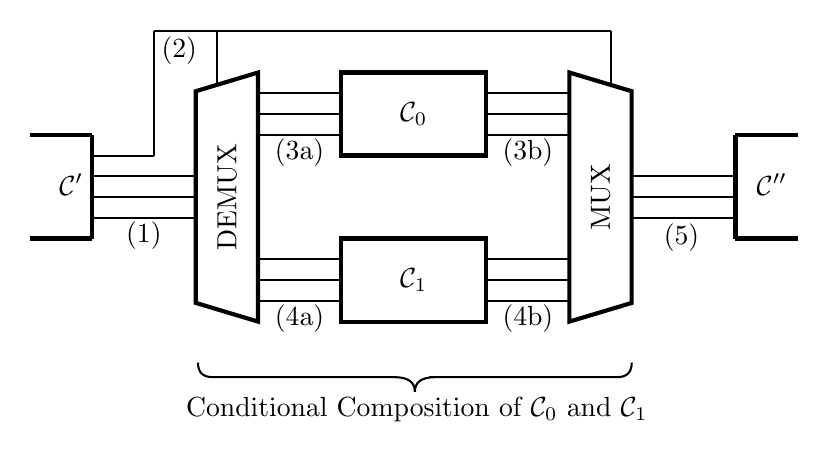
\begin{tikzpicture}[x=0.75pt,y=0.75pt,yscale=-1,xscale=1]
%uncomment if require: \path (0,259.75); %set diagram left start at 0, and has height of 259.75

%Shape: Rectangle [id:dp4766961530183158] 
\draw  [line width=1.5]  (180,50) -- (250,50) -- (250,90) -- (180,90) -- cycle ;
%Shape: Rectangle [id:dp6395866395594721] 
\draw  [line width=1.5]  (180,130) -- (250,130) -- (250,170) -- (180,170) -- cycle ;
%Shape: Trapezoid [id:dp22099663523420177] 
\draw  [line width=1.5]  (140,170) -- (110,161) -- (110,59) -- (140,50) -- cycle ;
%Shape: Trapezoid [id:dp22807725243960708] 
\draw  [line width=1.5]  (290,50) -- (320,59) -- (320,161) -- (290,170) -- cycle ;
%Straight Lines [id:da8367112919212248] 
\draw    (140,60) -- (180,60) ;


%Straight Lines [id:da7407114689901518] 
\draw    (140,70) -- (180,70) ;


%Straight Lines [id:da3819240715789862] 
\draw    (140,80) -- (180,80) ;


%Straight Lines [id:da009863437788521834] 
\draw    (140,140) -- (180,140) ;


%Straight Lines [id:da10678449062552275] 
\draw    (140,150) -- (180,150) ;


%Straight Lines [id:da6870537535345183] 
\draw    (140,160) -- (180,160) ;


%Straight Lines [id:da6742713516891087] 
\draw    (250,60) -- (290,60) ;


%Straight Lines [id:da4491705121978231] 
\draw    (250,70) -- (290,70) ;


%Straight Lines [id:da15578636910241705] 
\draw    (250,80) -- (290,80) ;


%Straight Lines [id:da8389085289883094] 
\draw    (250,140) -- (290,140) ;


%Straight Lines [id:da17359313640848217] 
\draw    (250,150) -- (290,150) ;


%Straight Lines [id:da7245129947221103] 
\draw    (250,160) -- (290,160) ;


%Straight Lines [id:da8860980928886597] 
\draw    (60,100) -- (110,100) ;


%Straight Lines [id:da2214036489357475] 
\draw    (60,90) -- (90,90) ;


%Straight Lines [id:da782884223107178] 
\draw    (60,110) -- (110,110) ;


%Straight Lines [id:da2886885602626673] 
\draw    (60,120) -- (110,120) ;


%Straight Lines [id:da002379315845792873] 
\draw    (90,30) -- (90,90) ;


%Straight Lines [id:da7039251112323563] 
\draw    (90,30) -- (310,30) ;


%Straight Lines [id:da6226435185112744] 
\draw    (120,30) -- (120,56) ;


%Straight Lines [id:da7950616134115784] 
\draw    (310,30) -- (310,56) ;


%Straight Lines [id:da518677667737772] 
\draw [line width=1.5]    (60,80) -- (60,130) ;


%Straight Lines [id:da9062917439017146] 
\draw [line width=1.5]    (60,130) -- (30,130) ;


%Straight Lines [id:da991274741569332] 
\draw [line width=1.5]    (60,80) -- (30,80) ;


%Straight Lines [id:da11931869210343404] 
\draw [line width=1.5]    (400,130) -- (370,130) ;


%Straight Lines [id:da39682448457779085] 
\draw [line width=1.5]    (400,80) -- (370,80) ;


%Straight Lines [id:da710175113163307] 
\draw    (320,100) -- (370,100) ;


%Straight Lines [id:da86316125759135] 
\draw    (320,110) -- (370,110) ;


%Straight Lines [id:da7803220671597932] 
\draw    (320,120) -- (370,120) ;


%Straight Lines [id:da43100575394299256] 
\draw [line width=1.5]    (370,80) -- (370,130) ;


%Shape: Brace [id:dp7065929076241165] 
\draw   (111.04,189.76) .. controls (111.04,194.43) and (113.37,196.76) .. (118.04,196.76) -- (205.54,196.76) .. controls (212.21,196.76) and (215.54,199.09) .. (215.54,203.76) .. controls (215.54,199.09) and (218.87,196.76) .. (225.54,196.76)(222.54,196.76) -- (313.04,196.76) .. controls (317.71,196.76) and (320.04,194.43) .. (320.04,189.76) ;

% Text Node
\draw (215,70) node  [align=left] {$\displaystyle \mathcal{C}_{0}$};
% Text Node
\draw (215,150) node  [align=left] {$\displaystyle \mathcal{C}_{1}$};
% Text Node
\draw (125,110) node [rotate=-270] [align=left] {DEMUX};
% Text Node
\draw (305,110) node [rotate=-270] [align=left] {MUX};
% Text Node
\draw (216.5,212.5) node  [align=left] {Conditional Composition of $\displaystyle \mathcal{C}_{0}$ and $\displaystyle \mathcal{C}_{1}$};
% Text Node
\draw (85,128.5) node [color={rgb, 255:red, 0; green, 0; blue, 0 }  ,opacity=1 ] [align=left] {(1)};
% Text Node
\draw (102,39.5) node [color={rgb, 255:red, 0; green, 0; blue, 0 }  ,opacity=1 ] [align=left] {(2)};
% Text Node
\draw (160,88.5) node [color={rgb, 255:red, 0; green, 0; blue, 0 }  ,opacity=1 ] [align=left] {(3a)};
% Text Node
\draw (270,88.5) node [color={rgb, 255:red, 0; green, 0; blue, 0 }  ,opacity=1 ] [align=left] {(3b)};
% Text Node
\draw (160,168.5) node [color={rgb, 255:red, 0; green, 0; blue, 0 }  ,opacity=1 ] [align=left] {(4a)};
% Text Node
\draw (270,168.5) node [color={rgb, 255:red, 0; green, 0; blue, 0 }  ,opacity=1 ] [align=left] {(4b)};
% Text Node
\draw (344,129.5) node [color={rgb, 255:red, 0; green, 0; blue, 0 }  ,opacity=1 ] [align=left] {(5)};
% Text Node
\draw (50,104) node  [align=left] {$\displaystyle \mathcal{C} '$};
% Text Node
\draw (387.5,104) node  [align=left] {$\displaystyle \mathcal{C} ''$};


\end{tikzpicture}


